% The design of the software (using a combination of diagrams and words)

\subsection{Design}

\subsubsection{Overview}

The software shall be designed using a primarily functional approach. The core of the algorithm shall be created in a module named \texttt{viperCrypt}. Normal interaction with the module shall occur by calling the \texttt{crypt()} function (See \nameref{cryptOverview}) and passing the user key, the plain-- or cipher--text, and a flag, which indicates whether to encrypt or decrypt. The \texttt{crypt()} function shall return the result of the encryption or decryption.

\begin{figure}[H]
\centering
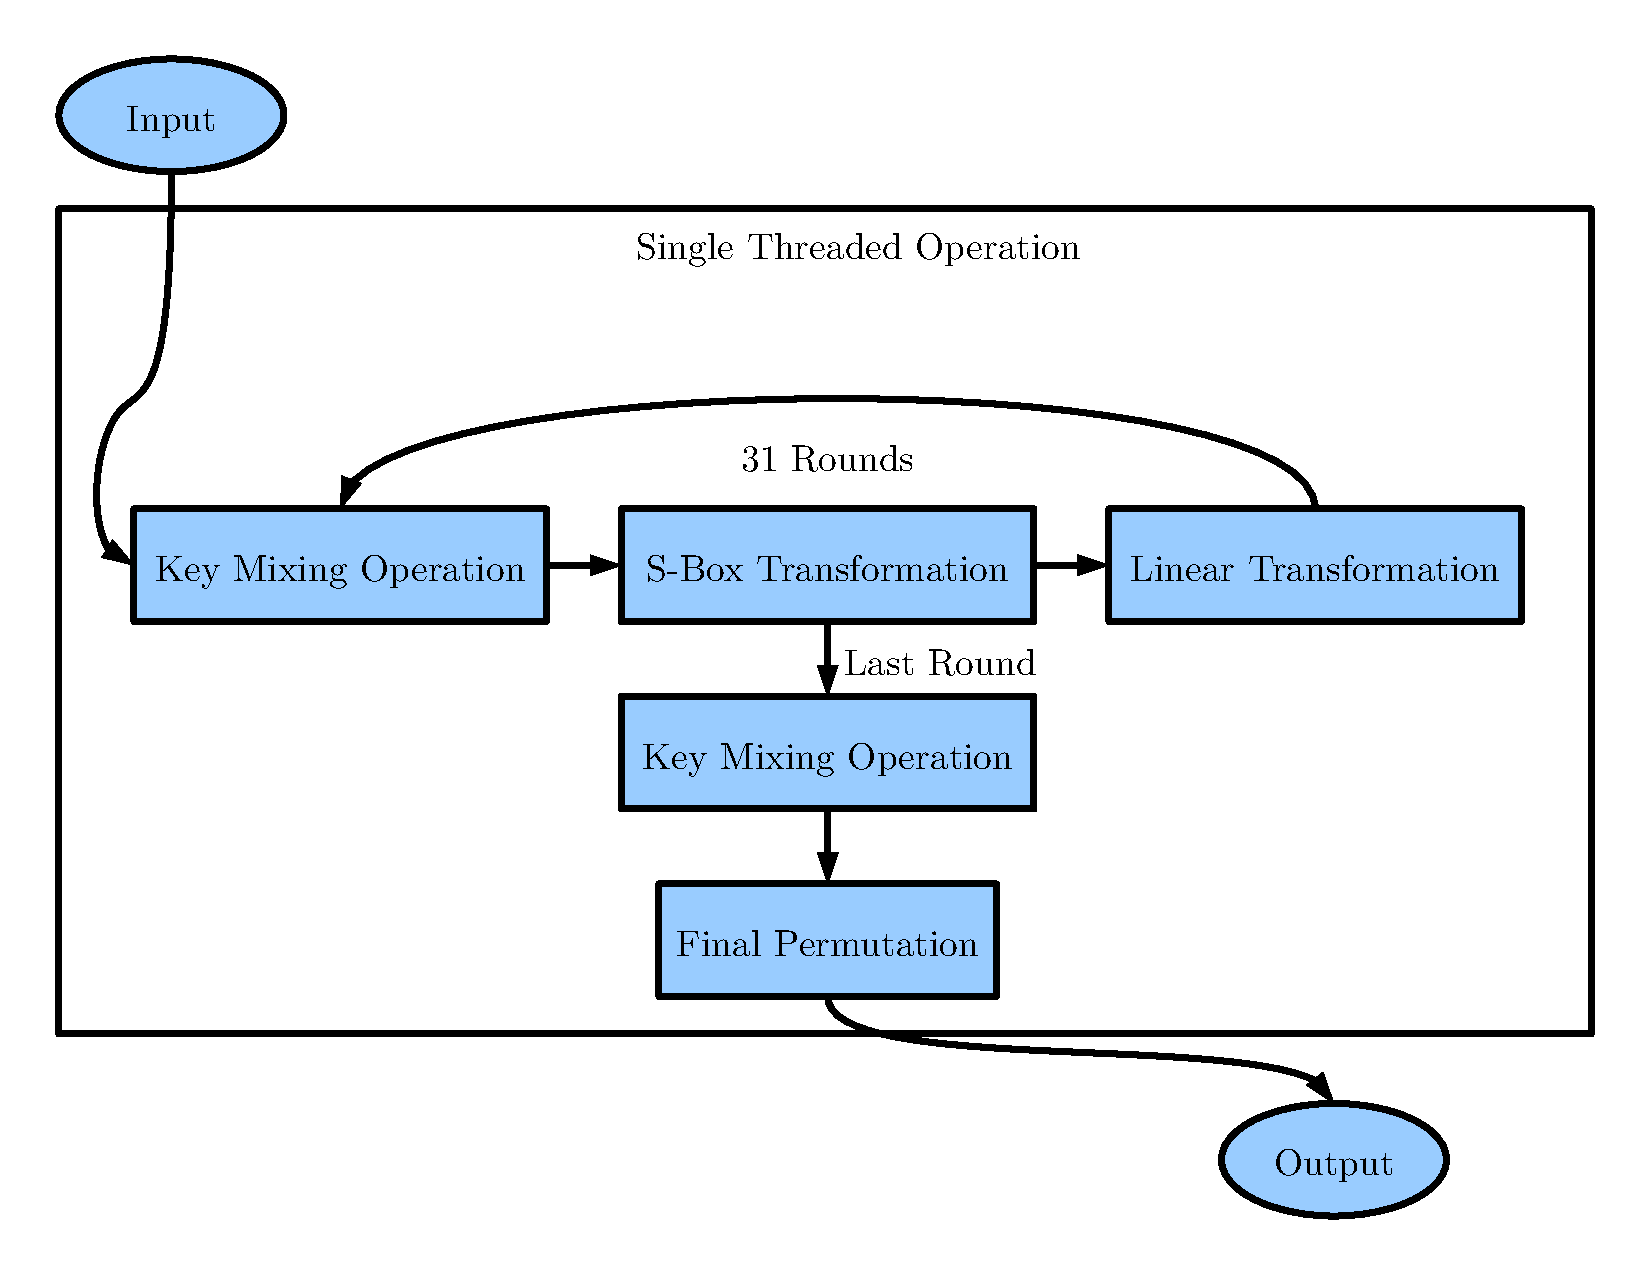
\includegraphics[width=0.8\textwidth]{Design-Overview-Cipher.pdf}
\caption{Dataflow Diagram}
\label{cryptOverview}
\end{figure}

\subsubsection{Multi--Threading}

The multi--threaded version of \texttt{Viper} shall be implemented as 32 threads (See \nameref{threadedOverview}), where each thread consists of \texttt{viperCrypt.crypt()} operating on a separate block of input data.

\begin{figure}[H]
\centering
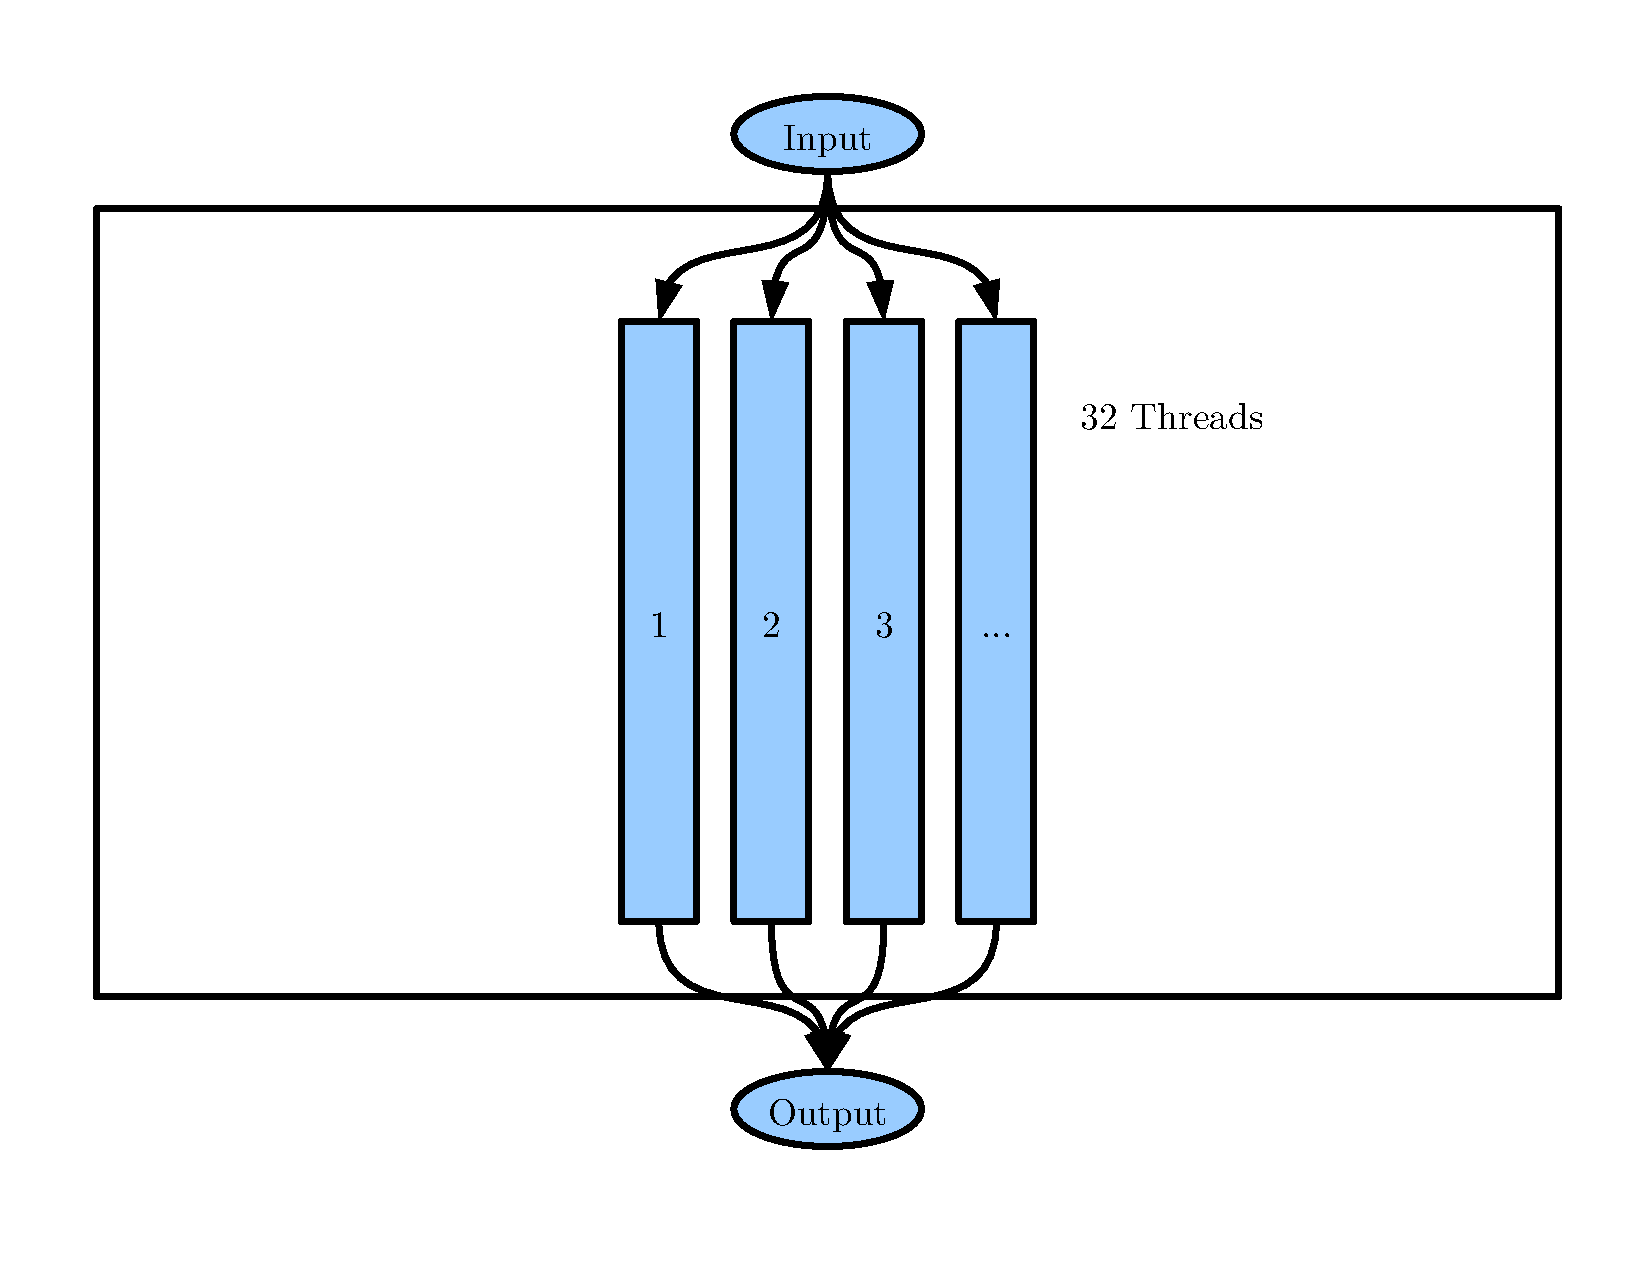
\includegraphics[width=0.8\textwidth]{Design-Overview-Threaded.pdf}
\caption{Threaded Dataflow Diagram}
\label{threadedOverview}
\end{figure}
